\documentclass{article}
\usepackage[utf8]{inputenc}
\usepackage[letterpaper, portrait, margin=0.5in]{geometry}
\usepackage{multicol}
\usepackage{graphicx}
\graphicspath{ {../images} }

\begin{document}

\begin{center}
\large
Chemistry 130 Kinetics Reference Sheet\\
\normalsize
Reese Critchlow, 2021
\begin{multicols}{3}

    \large
    \textbf{Zeroth Order}
    \normalsize
    \medskip
    
    \underline{Rate}
    \[
        \textrm{Rate} = \frac{-d\textrm{[A]}}{dt} = k
    \]
    
    \underline{Integrated Rate Law}
    \[
        \textrm{[A]}_t  - \textrm{[A]}_0 = -kt
    \]

    \underline{Half Life}
    \[
        t_{\frac{1}{2}} = \frac{\textrm{[A]}_0}{2k}
    \]
    \footnotesize
    Half Life Decreases With Time
    \normalsize\\
    \medskip
    \underline{Plot}
    \[
        \textrm{[A]}_t = -kt + \textrm{[A]}_0
    \]
    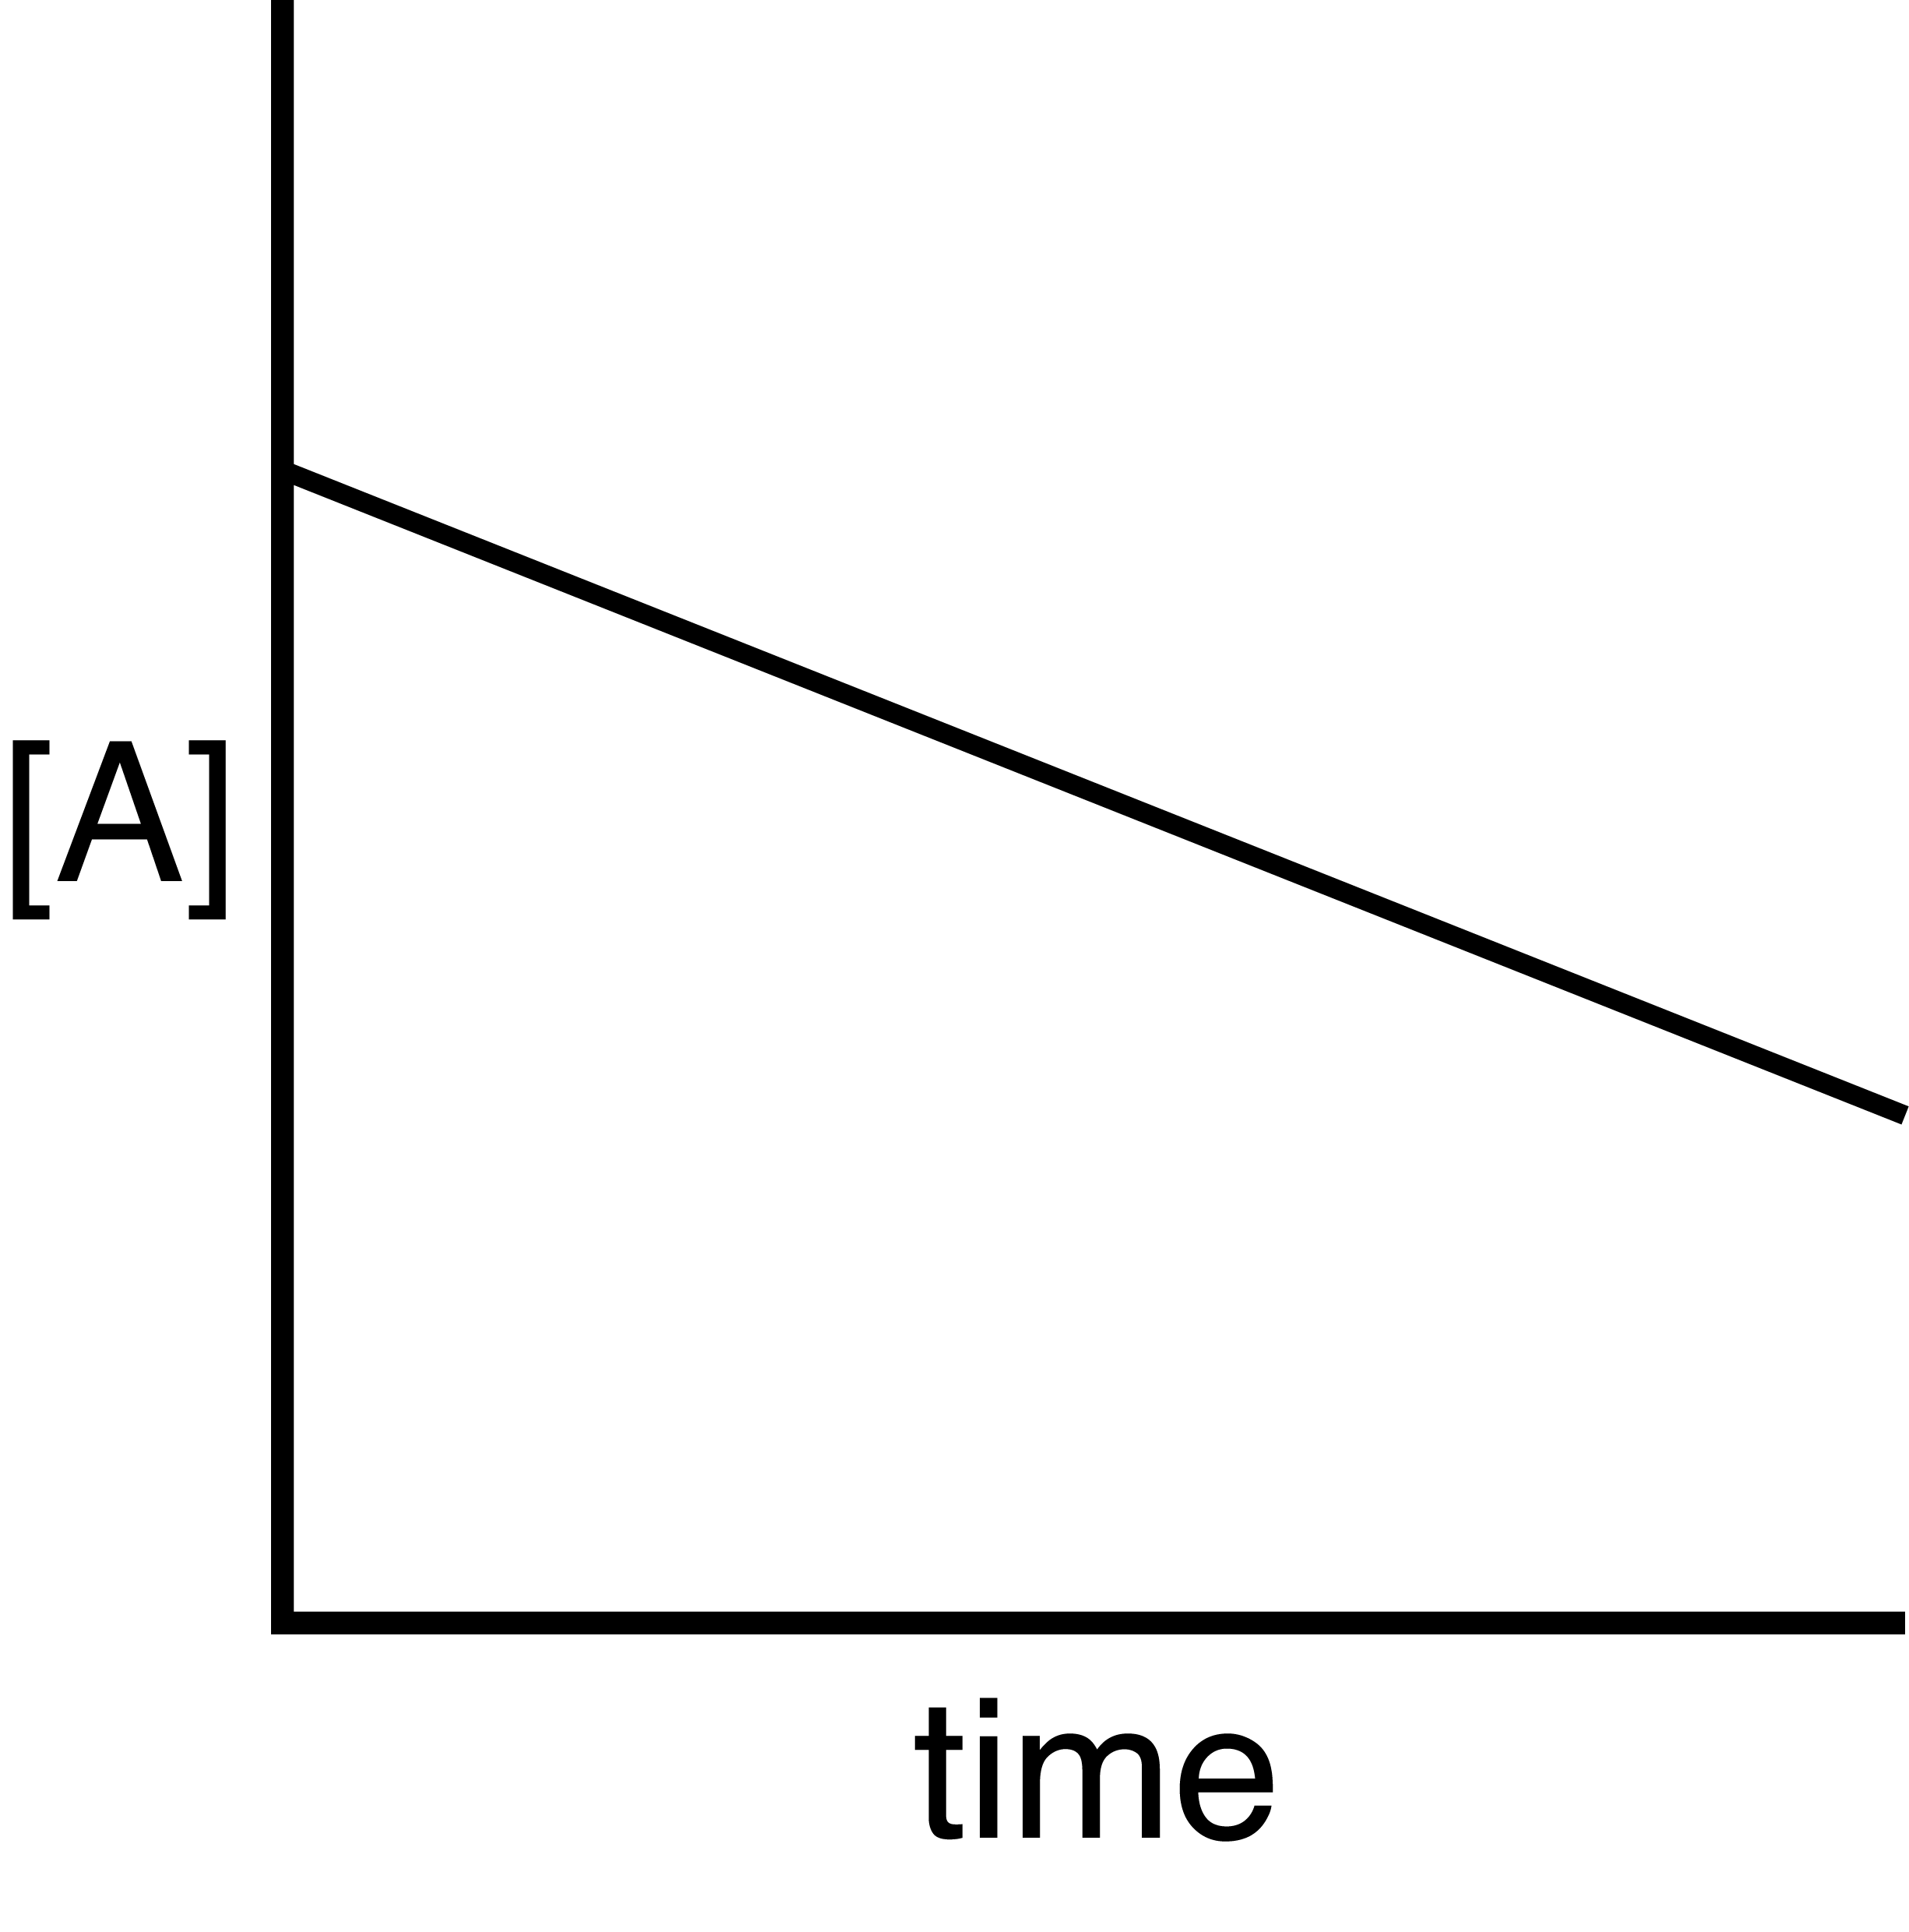
\includegraphics[scale =0.25]{zerothorder.png}
    
    


\vfill\null\columnbreak

    \large
    \textbf{First Order}
    \normalsize
    \medskip
    
    \underline{Rate}
    \[
        \textrm{Rate} = \frac{-d\textrm{[A]}}{dt} = k\textrm{[A]}
    \]
    
    \underline{Integrated Rate Law}
    \[
        \ln{\textrm{[A]}_t} - \ln{\textrm{[A]}_0} = -kt
    \]
    - or -
    \[
        \frac{\textrm{[A]}_t}{\textrm{[A]}_0} = e^{-kt}
    \]
    
    \underline{Half Life}
    \[
        t_{\frac{1}{2}} = \frac{\ln{2}}{k}
    \]
    \footnotesize
    Half Life is Independent of Time
    \normalsize\\
    \medskip
    \underline{Plot}
    \[
        \ln{\textrm{[A]}_t} = -kt + \ln{\textrm{[A]}_0}
    \]
    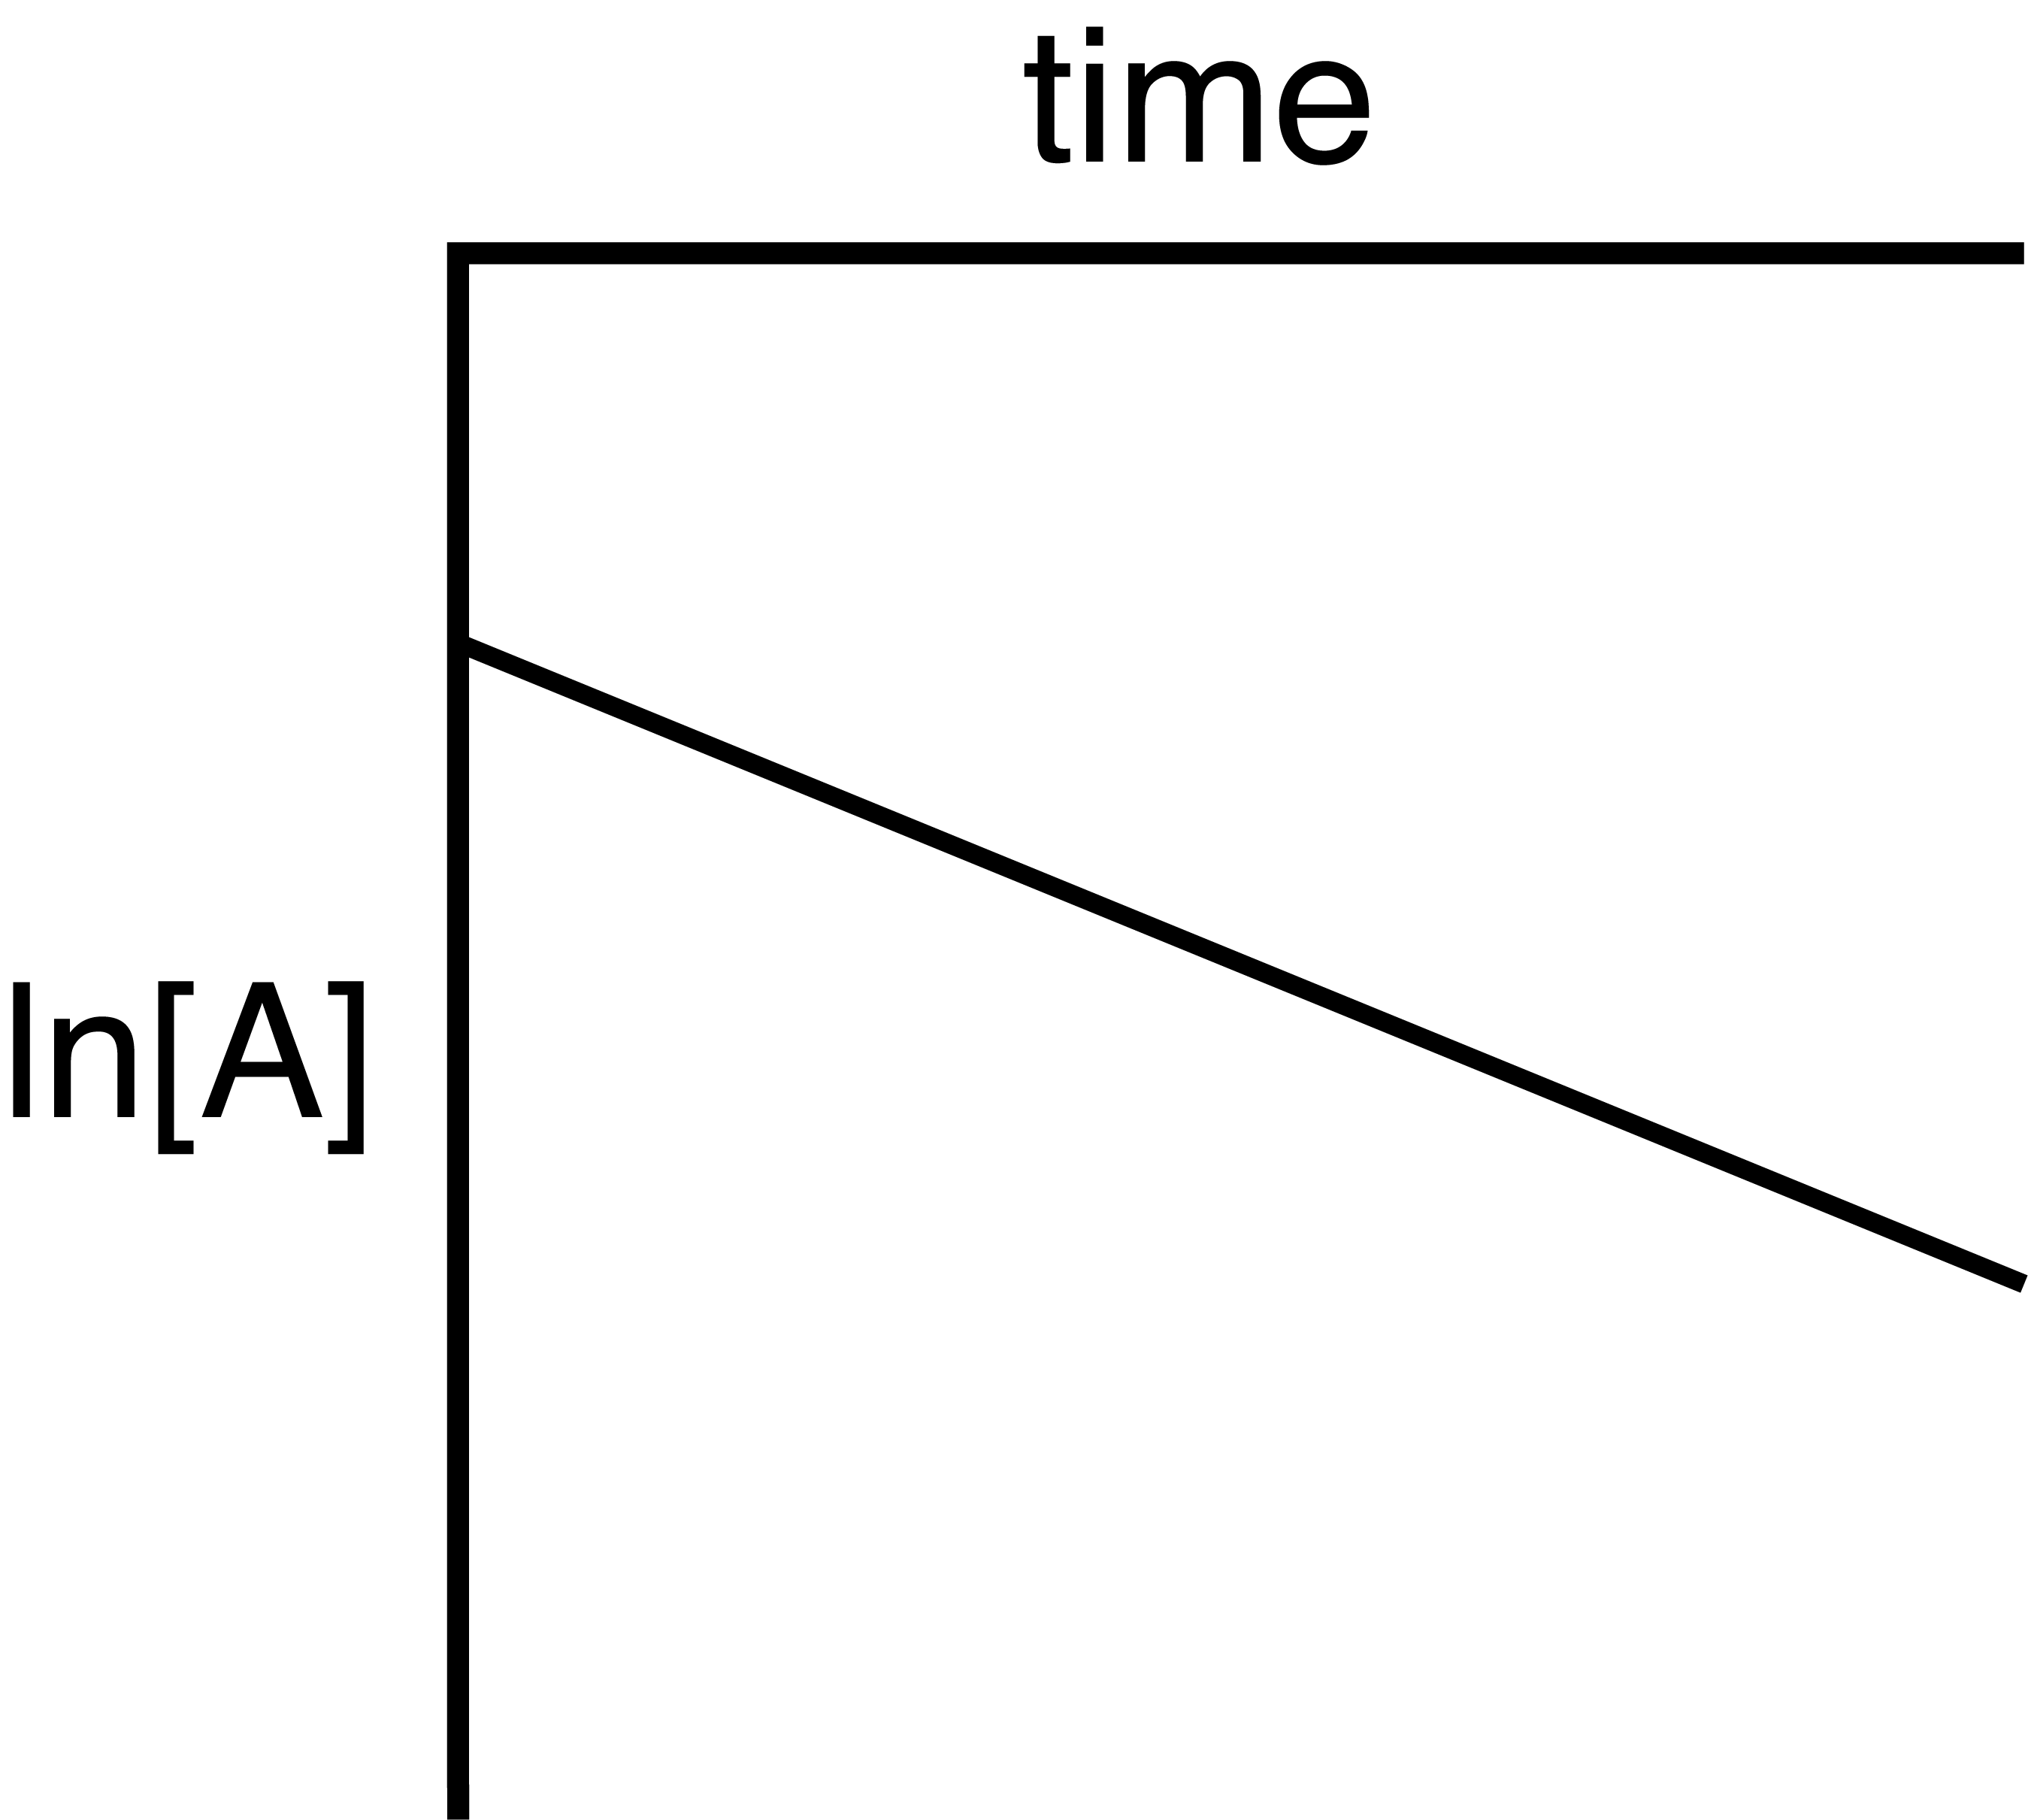
\includegraphics[scale =0.25]{secondorder.png}
    
\vfill\null\columnbreak

    \large
    \textbf{Second Order}
    \normalsize
    \medskip
    
    \underline{Rate}
    \[
        \textrm{Rate} = \frac{-1}{2}\frac{d\textrm{[A]}}{dt} = \frac{d\textrm{[B]}}{dt} = k_1\textrm{[A]}^2 \quad (1)
    \]
    - or -
    \[
        \textrm{Rate} = \frac{-d\textrm{[A]}}{dt} = k_2\textrm{[A]}^2 \qquad \qquad \quad (2)
    \]
    
    \underline{Integrated Rate Law}
    \[
        \frac{1}{\textrm{[A]}_t} = 2k_1t + \frac{1}{\textrm{[A]}_0} \qquad (1)
    \]
    - or -
    \[
        \frac{1}{\textrm{[A]}_t} = k_2t + \frac{1}{\textrm{[A]}_0} \qquad (2)
    \]
    
    \underline{Half Life}
    \[
        t_{\frac{1}{2}} = \frac{1}{k\textrm{[A]}_0}
    \]
    \footnotesize
    Half Life is Independent of Time
    \normalsize\\
    \medskip
    \underline{Plot}
    \[
        \frac{1}{\textrm{[A]}_t} = kt + \frac{1}{\textrm{[A]}_0}
    \]
    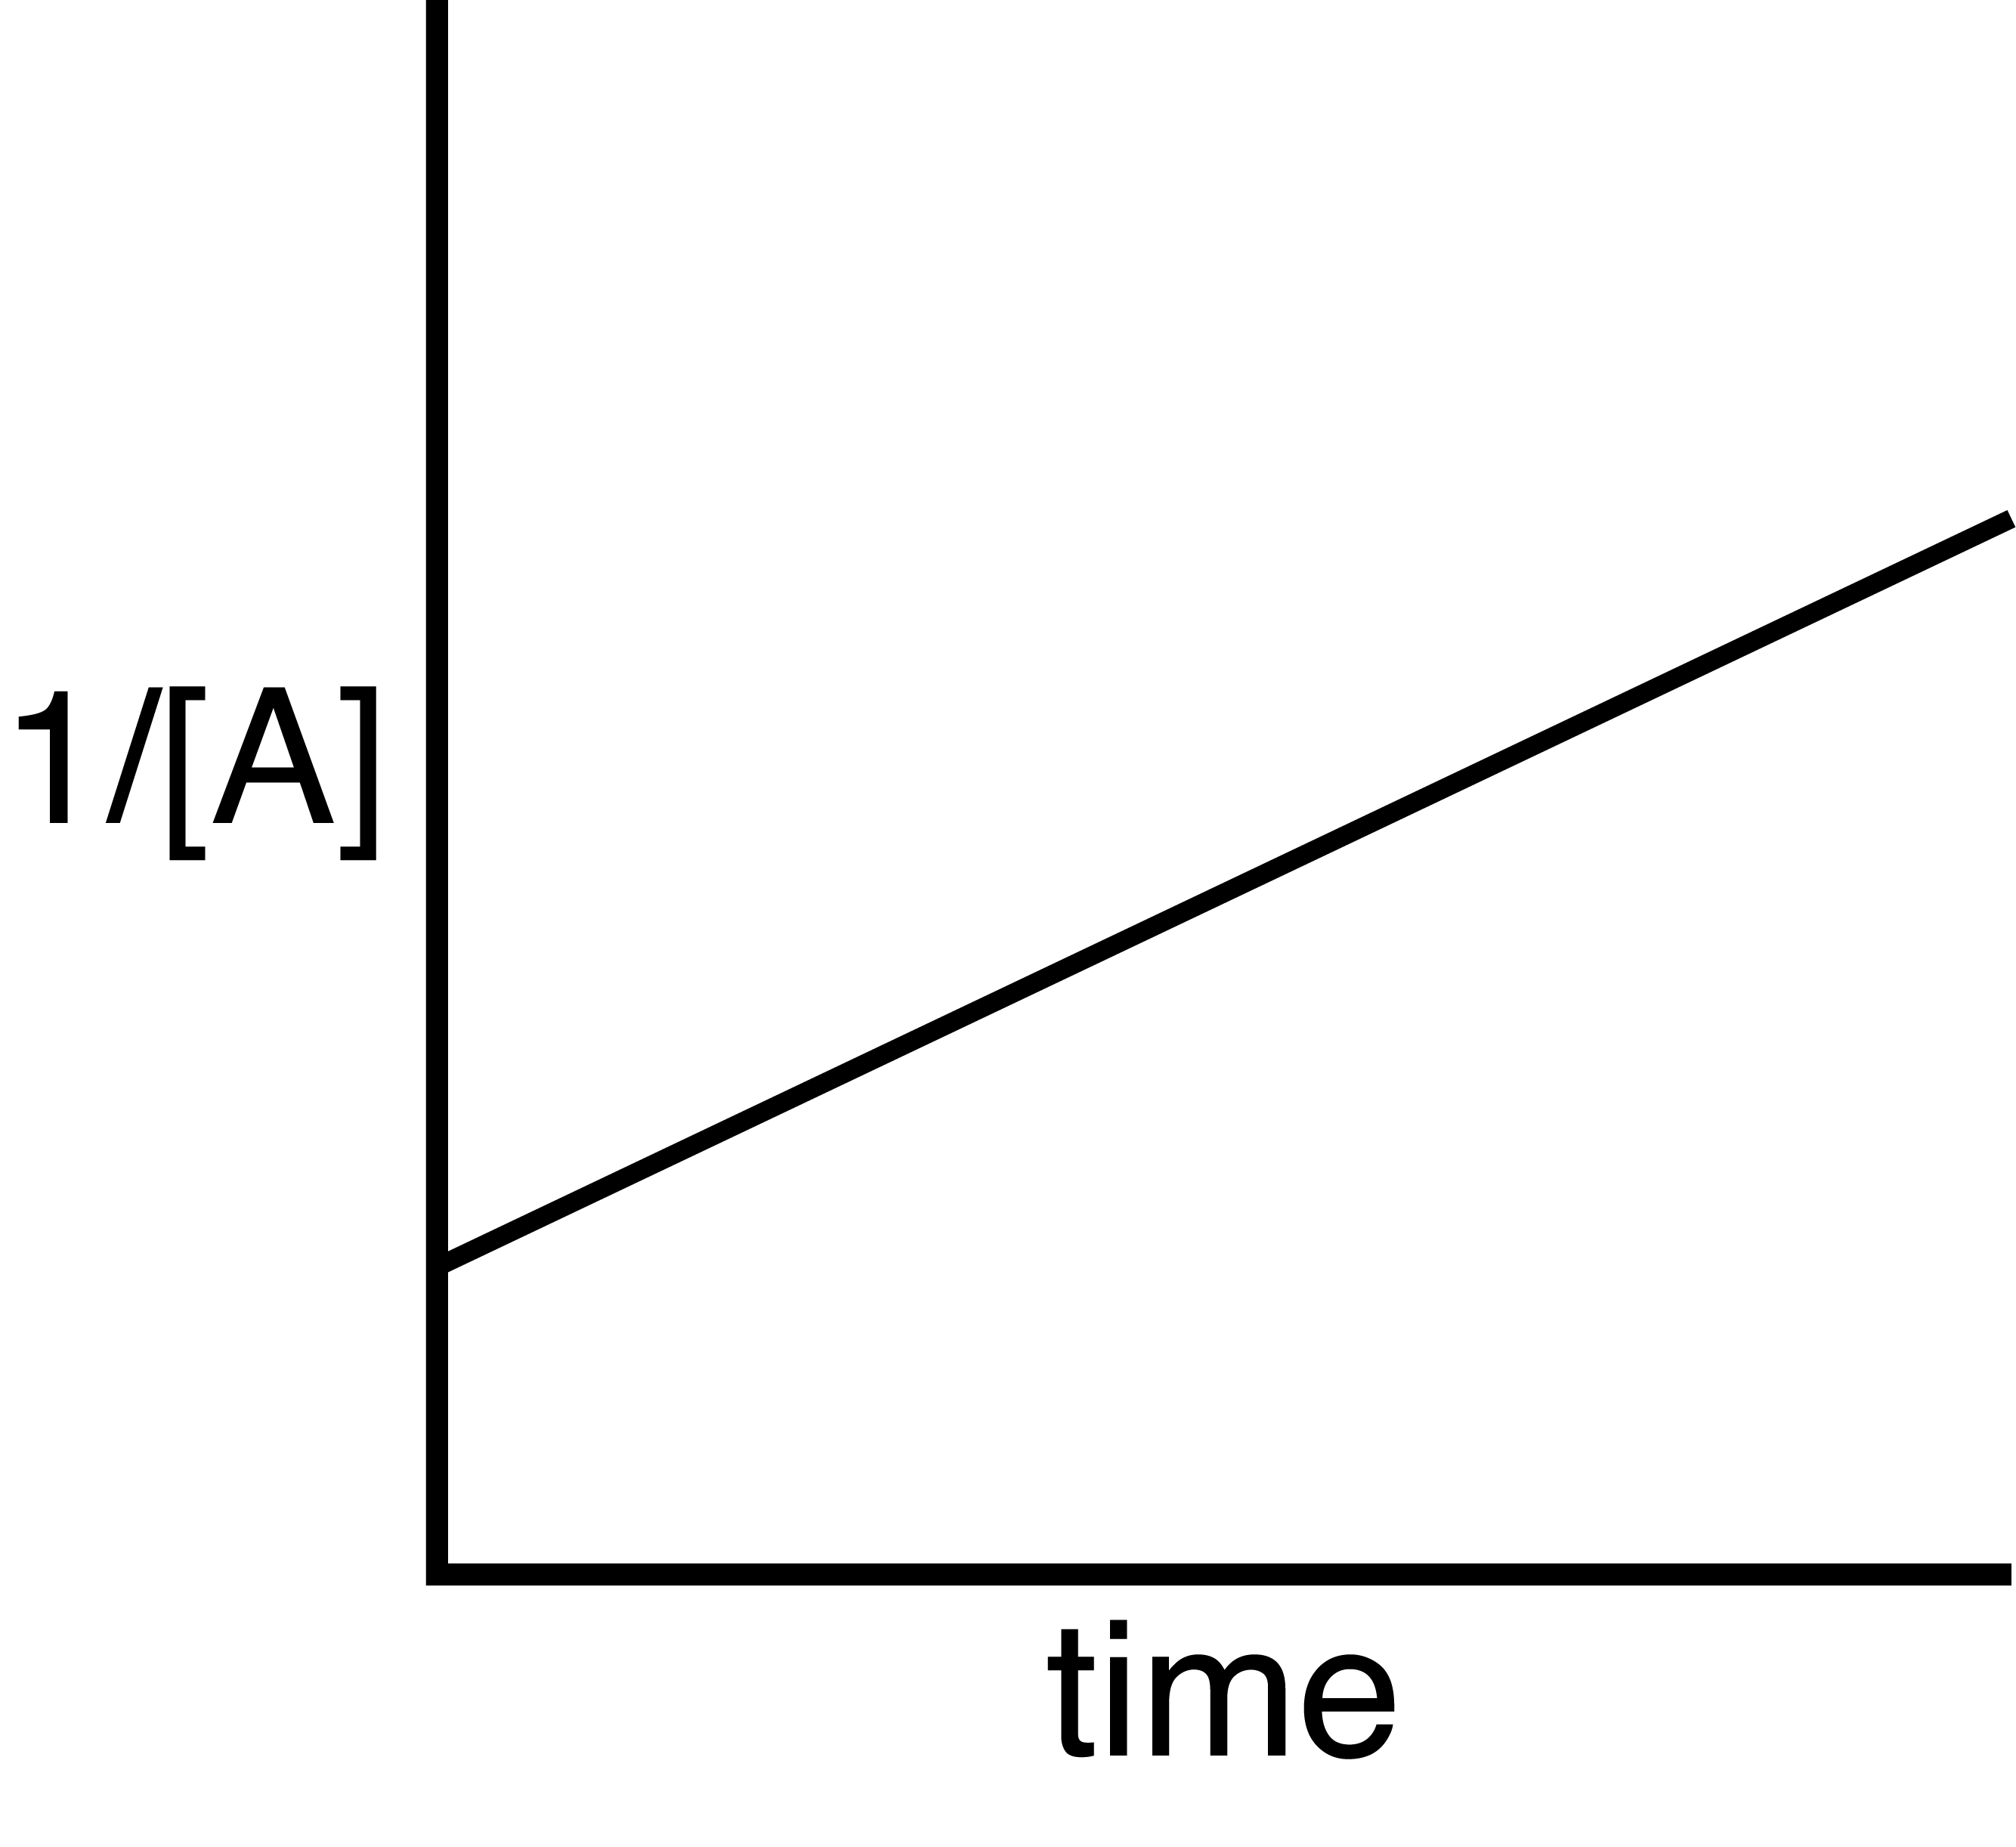
\includegraphics[scale =0.25]{firstorder.png}

\end{multicols}
\begin{large}
\textbf{Other Formulae for Kinetics}
\end{large}

\begin{multicols}{2}
    
    \underline{Arrhenius Equation}
    \[
        k = Ae^{\frac{-E_a}{RT}}
    \]
    
    \underline{Arrhenius Plot Equation}
    \[
        \frac{\Delta\ln{k}}{\Delta\left(\frac{1}{T}\right)} = \frac{-E_a}{R}
    \]
    
\end{multicols}

\end{center}

\end{document}
